\documentclass{article} 
 \usepackage{tikz} 
 \usetikzlibrary{trees} 
 \begin{document} 


 \begin{frame} 

 
\begin{tikzpicture}[level distance=2cm, level 1/.style={sibling distance=7cm}, level 2/.style={sibling distance=3.5cm}, level 3/.style={sibling distance=2cm}] 
\node [circle,draw,thick] {3}; 
 \end{tikzpicture} 

 \end{frame} 

 \newpage
 \begin{frame} 

 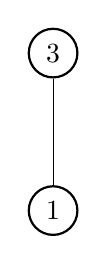
\begin{tikzpicture}[level distance=2cm, level 1/.style={sibling distance=7cm}, level 2/.style={sibling distance=3.5cm}, level 3/.style={sibling distance=2cm}] 
\node [circle,draw,thick] {3}
 child {node [circle,draw,thick] {1}}; 
 \end{tikzpicture} \end{frame} 

 \newpage
 \begin{frame} 

 \begin{tikzpicture}[level distance=2cm, level 1/.style={sibling distance=7cm}, level 2/.style={sibling distance=3.5cm}, level 3/.style={sibling distance=2cm}] 
\node [circle,draw,thick] {3}
 child {node [circle,draw,thick] {1}}
 child {node [circle,draw,thick] {4}}; 
 \end{tikzpicture} \end{frame} 

 \newpage
 \end{document} 
